\documentclass[11pt,toc=bibliography]{scrbook}
\usepackage[utf8]{inputenc}
\usepackage[mode=buildnew]{standalone}
\usepackage{amsmath}
\usepackage{amssymb}
\usepackage{mathtools}
\usepackage{braket}
\usepackage[svgnames,dvipsnames]{xcolor}
\usepackage{graphicx}
\usepackage{adjustbox}
\usepackage{cite}
\usepackage{calc}
\usepackage[subrefformat=parens]{subcaption}
\usepackage[titletoc]{appendix}
\usepackage[colorlinks, linktocpage, hypertexnames = false]{hyperref}
\usepackage{authblk}

%%% inkscapefig https://github.com/sleepymalc/VSCode-LaTeX-Inkscape
\usepackage{import}
\usepackage{svg}
\usepackage{xifthen}
\usepackage{pdfpages}
\usepackage{transparent}
\usepackage{relsize}
\usepackage{booktabs}

\newcommand{\incfig}[2][]{%
    %\def\svgwidth{\columnwidth}
    \includeinkscape[#1]{#2.pdf_tex}
}

\pdfsuppresswarningpagegroup=1
%%% inkscapefig end

%itemize vertical spaces
\usepackage{enumitem}
\setitemize{itemsep=0pt}

% Layout
\RequirePackage[top=12mm,bottom=12mm,left=30mm,right=30mm,head=12mm,includeheadfoot]{geometry}
\bigskipamount 6mm

%KO's macro
%\usepackage{fusioncat}
\DeclareMathOperator{\vol}{vol}
\DeclareMathOperator{\U}{U}
\DeclareMathOperator{\SU}{SU}
\DeclareMathOperator{\imunit}{i}
\DeclareMathOperator{\id}{id}
\DeclareMathOperator{\Map}{Map}
\newcommand{\stdim}{D}

%blackboard one
\usepackage{dsfont}
\newcommand{\bbone}{I}

%title font to small capitals
\setkomafont{title}{\normalcolor\scshape}

%quiver
\usepackage{quiver}

%%% path to figures
\graphicspath{{figures/}}


%%% pdf version
%\pdfminorversion=7


\hypersetup{linkcolor = Crimson, citecolor = MediumBlue, urlcolor = MediumBlue}

\numberwithin{equation}{section}

\newcommand{\bigboxplus}{
  \mathop{
    \vphantom{\bigoplus} 
    \mathchoice
      {\vcenter{\hbox{\resizebox{\widthof{$\displaystyle\bigoplus$}}{!}{$\boxplus$}}}}
      {\vcenter{\hbox{\resizebox{\widthof{$\bigoplus$}}{!}{$\boxplus$}}}}
      {\vcenter{\hbox{\resizebox{\widthof{$\scriptstyle\oplus$}}{!}{$\boxplus$}}}}
      {\vcenter{\hbox{\resizebox{\widthof{$\scriptscriptstyle\oplus$}}{!}{$\boxplus$}}}}
  }\displaylimits 
}

%the notation for the category after gauging M
\newcommand{\gaugedcat}[2]{#1_{#2}}

%includestandalone in a raisebox to align the baseline
\newcommand*{\includestandaloneraise}[2][]{\raisebox{-.5\height}{\includestandalone[#1]{#2}}}

%fixme
\usepackage[status=draft,inline,nomargin]{fixme}
\fxusetheme{color}
\FXRegisterAuthor{ko}{ako}{KO}
\FXRegisterAuthor{ki}{aki}{\color{red}KI}

%icons
\usepackage{fontawesome5}

%tcolorbox
\usepackage[most]{tcolorbox}
\tcbuselibrary{skins,breakable}

%%note
\newtcolorbox{note}[2][]{breakable,sharp corners, skin=enhancedmiddle jigsaw,parbox=false,
boxrule=0mm,leftrule=2mm,boxsep=0mm,arc=0mm,outer arc=0mm,attach title to upper,
after title={ \\}, coltitle=black, colback=blue!7,colframe=blue, title=\ifthenelse{\equal{#2}{}}{Note}{#2},
fonttitle=\sffamily\bfseries, before title ={\faPen\hspace{.3em}},#1}

%%important
\newtcolorbox{important}[2][]{breakable,sharp corners, skin=enhancedmiddle jigsaw,parbox=false,
boxrule=0mm,leftrule=2mm,boxsep=0mm,arc=0mm,outer arc=0mm,attach title to upper,
after title={ \\}, coltitle=black, colback=OrangeRed!7,colframe=OrangeRed, title=\ifthenelse{\equal{#2}{}}{Important}{#2},
fonttitle=\sffamily\bfseries, before title ={\faExclamation\hspace{.3em}},#1}

%%warning
\newtcolorbox{warning}[2][]{breakable,sharp corners, skin=enhancedmiddle jigsaw,parbox=false,
boxrule=0mm,leftrule=2mm,boxsep=0mm,arc=0mm,outer arc=0mm,attach title to upper,
after title={ \\}, coltitle=black, colback=orange!7,colframe=orange, title=\ifthenelse{\equal{#2}{}}{Warning}{#2},
fonttitle=\sffamily\bfseries, before title ={\faExclamationTriangle\hspace{.3em}},#1}

%longtable
\usepackage{longtable}

%tightlist
\providecommand{\tightlist}{%
  \setlength{\itemsep}{0pt}\setlength{\parskip}{0pt}}

\title{A Lecture on Topological Operators}
\author[1]{Kantaro Ohmori}
\affil[1]{Department of Physics, The University of Tokyo, Bunkyo-ku, Tokyo 113-0033, Japan}
\date{}

\begin{document}

\maketitle

\addchap*{Abstract}
AAA

\setcounter{page}{0}

\thispagestyle{empty}

\newpage

\tableofcontents

\flushbottom

\chapter{Introduction}

\section{Symmetry}

\textbf{Symmetry} plays a crucial role in theoretical physics. In this lecture, we will discuss its application in \emph{quantum field theories} (QFTs). A fundamental aspect of symmetry in QFTs is its preservation along the renormalization group flow. More precisely, when an ultraviolet (UV) theory \(\mathcal{T}_\text{UV}\) transitions into an infrared (IR) theory \(\mathcal{T}_\text{IR}\), a canonical homomorphism \(f_\text{RG}\) exists from the UV symmetry group \(G_\text{UV}\) to the IR symmetry group \(G_\text{IR}\):\footnote{If the UV theory is a fixed point, \(G_\text{UV}\) should be understood as the one preserved by the deformation triggering the RG flow. If the RG flow is to a lower nonzero energy, and if one retains all the (even very massive) degrees of freedom, and also all the irrelevant interactions in the description of \(\mathcal{T}_\text{IR}\), the map \(f_\text{RG}\) is an isomorphism. However, typically one integrates out massive degrees of freedom in the description of \(\mathcal{T}_\text{IR}\), in which case some symmetry can decouple and thus \(f_\text{RG}\) can be non-surjective. Also, if one drops some higher-order interaction terms, or runs the flow to zero energy, there can be an \emph{emergent} symmetry, in which case \(f_\text{RG}\) can be non-injective.}

\begin{important}{Symmetry matching along an RG flow}
  \begin{equation}
    f_\text{RG} : G_\text{UV} \to G_\text{IR}.
  \end{equation}
\end{important}

Given this relationship, symmetry in QFTs can be applied in two ways:

\begin{itemize}
  \tightlist
  \item UV to IR: Starting with a microscopic model (e.g., a model of elementary particles or electrons in matter), we can use symmetry to constrain or predict what happens on a macroscopic scale.
  \item IR to UV: Given certain macroscopic phenomena, we can use symmetry to constrain or infer the possible microscopic origins (e.g., inferring the QCD Lagrangian from the hadron spectrum).
\end{itemize}


\section{Locality}

One of the defining characteristics of symmetry in quantum field theories (QFTs) is its \emph{preservation of locality}. In the context of classical symmetry in fields, this means that the symmetry transformation is local:

\begin{equation}
  \phi(x) \mapsto F(\phi(x')),
  \label{eq: field-transform}
\end{equation}

In this equation, \(F(\phi(x'))\) is a function that relies solely on the \emph{local} value of a field (or a set of fields and its derivatives) at a point \(x'\). When \(x'\neq x\), the symmetry involves a \emph{spacetime} symmetry, while when \(x'=x\), it is an \emph{internal} symmetry. The preservation of locality in a symmetry underpins the symmetry relation in Eq.~\eqref{eq-RG-group-match}, which will be elaborated further in the lecture.

\begin{note}{}
  Please note that a QFT, when quantized on a fixed space manifold \(M\), possesses unitary operators that commute with its Hamiltonian, other than those originating from locality-preserving symmetry. In most cases, such unitary operators are irrelevant; an example is one that multiplies a phase to a specific eigenstate. Therefore, in this lecture, when we refer to a symmetry, we assume that it preserves locality. In fact, we assert that this property is the \emph{last} one to be discarded in the context of generalized symmetry, if ever, due to the invariance under renormalization group flow.\footnotemark{}
\end{note}

\footnotetext{Also, note that the Coleman-Mandula theorem assumes a strong locality-preserving condition; that the symmetry generators act on multi-particle asymptotic states as tensor products.}

\begin{note}{}
  To avoid confusion, it's important to note that locality-preserving symmetry does \emph{not} mean gauge redundancy, which is sometimes labeled as local symmetry. The global -- spacetime, or internal -- symmetries typically encountered in a QFT textbook all preserve locality.
\end{note}

However, not all symmetries in QFT that preserve locality take the form of Eq.~\eqref{eq: field-transform}, i.e., a \emph{classical} symmetry. Other types of symmetries exist, such as \emph{topological symmetry} or \emph{quantum symmetry}, which emerge from topologically nontrivial field configurations. Examples include the winding symmetry in 1+1d compact boson, and the monopole symmetries in 2+1d abelian gauge theories. In many cases, a topological/quantum symmetry is mapped to a symmetry of the type in Eq.~\eqref{eq-field-transform} under a duality, and thus it should also be considered as preserving locality.

From a contemporary standpoint, the universal characterization of locality-preserving symmetries is their correspondence to \textbf{topological operators}. A topological operator \(\mathcal{D}[W_n]\) in a QFT is an extended operator defined on an \(n\)-dimensional submanifold of the spacetime. The correlators that include it should remain invariant under the smooth deformation of the supporting manifold \(W_n\) (See Figure~\ref{fig-TopOpsDeform}).

\begin{figure}[t]
  {\centering 
\includegraphics[width=\textwidth]{figures/TopOpsDeform.png} }
  \caption{\label{fig-TopOpsDeform}Topological operator.}
\end{figure}

The first goal of this lecture is to understand the following correspondence:

\begin{important}{Symmetry/topological operator correspondence 1}
  \begin{equation}
    \begin{split}
       & \text{(Conventional) locality-preserving symmetry} \\
       & \Longleftrightarrow\;
      \text{invertible topological operator of codimension 1.}
    \end{split}
    \label{eq: conv-STO-corresp}
  \end{equation}
\end{important}

In this correspondence, the topological operator should be viewed as a generalization of the \textbf{Noether charge} for potentially discrete symmetry. More precisely, we consider this correspondence as the right-hand side \emph{defining} the left-hand side. We will explicitly verify that this correspondence/definition reproduces the known symmetries in the case of a classical symmetry in a scalar field theory in Chapter~\ref{sec-scalar}, and in the case of abelian gauge theory in Chapter~\ref{sec-vector}. The case of fermions is both intriguing and crucial, but it will be left as an exercise, or a work, for the audience/readers.

\begin{warning}{Terminology: topological defect}
  There exists an unfortunate discrepancy in terminology. Outside the realm of generalized symmetry literature, a ``topological defect'' typically refers to a dynamical object, or its trajectory, viewed as an operator in the IR theory. As an operator in the IR theory, it is \emph{not} necessarily topological in the sense of Figure~\ref{fig-TopOpsDeform}. Instead, it is often an operator charg\emph{ed} under a (generalized) symmetry emanating from the topology of space of field configurations. Conversely, within the generalized symmetry literature, ``topological defect (operator)'' often signifies an extended operator that is  topological in the sense of Fig.~\ref{fig-TopOpsDeform} even in the microscopic model. To mitigate potential confusion in this lecture, we will adopt the term ``topological operator'', even when the supporting submanifold of the operator is not within a time-slice.
\end{warning}

\section{Generalized Symmetry}

The concept of \textbf{generalized (global) symmetry} is fundamentally
based on the correspondence in Eq.~\eqref{eq: conv-STO-corresp}, as
introduced by \cite{Gaiotto:2014kfa}\footnote{The concept of global
  higher-form symmetry has been previously explored and investigated in
  the literature, for example, in
  \cite{Kapustin:2013uxa,Barkeshli:2014cna}. Its gauged version was
  essentially known from \cite{KalbRamond}.}. This concept expands
the traditional notion of symmetry by loosening the constraints on the
right-hand side of Eq.~\eqref{eq: conv-STO-corresp}. Hence, we
\emph{define} generalized symmetry through the following correspondence,
which extends Eq.~\eqref{eq: conv-STO-corresp}:

\begin{important}{Symmetry/topological operator correspondence 2}
  \begin{equation}
    \begin{split}
      & \text{Generalized symmetry (in a ``usual" QFT)} \\
      & \stackrel{\text{def}}{\Longleftrightarrow}\;
      \text{General topological operator.}
      \label{eq: GSTO-corresp}
    \end{split}
  \end{equation}
\end{important}

In more specific terms, a generalized symmetry that corresponds to an
operator of codimension \(p+1\) is referred to as a \textbf{\(p\)-form
  symmetry}. Meanwhile, a generalized symmetry that corresponds to an
operator without an inverse is known as a \textbf{non-invertible
  symmetry} (also referred to as category symmetry or topological
symmetry).

In the context of an ``unusual'' QFT, the topological constraint on the
operator on the right-hand side of Eq.~\eqref{eq: GSTO-corresp} can be
further relaxed. This leads to the concept of \textbf{subsystem} and \textbf{dipole} 
symmetry, which will be briefly mentioned in
Section~\ref{sec-trivial-scalar}, but will not be discussed in detail in
this lecture.

Table \ref{tbl: sym-classes} summarizes the subclasses of generalized symmetry.
These subclasses are not mutually exclusive. Therefore, in theory, a
2-form non-invertible subsystem symmetry could exist, for example.

In the following chapters, we will explore the correspondence in Eq.~\eqref{eq: GSTO-corresp} in the context of scalar field theory and Abelian gauge theory. We focus on the explicit construction of the topological operators, and consequences we can derive from them. 

\begin{table}
\begin{longtable}[]{@{}llll@{}}
  \caption{\label{tbl: sym-classes}Subclasses of generalized symmetry and
    defining properties of their corresponding topological
    operators.}\tabularnewline
  \toprule\noalign{}
               & \(p\)-form & non-invertible & subsystem/dipole \\
  \midrule\noalign{}
  \endfirsthead
  \toprule\noalign{}
               & \(p\)-form & non-invertible & subsystem \\
  \midrule\noalign{}
  \endhead
  \bottomrule\noalign{}
  \endlastfoot
  codimension  & \(p+1\)    &                &           \\
  Invertible?  &            & No             &           \\
  Topological? &            &                & Partially \\
\end{longtable}
\end{table}

\chapter{Topological Operators for Classical Symmetry}
\label{sec-scalar}

This section explores topological operators in the context of classical symmetry in scalar field theory.

\section{Set Up}
For specificity, consider a complex scalar field theory with the following Lagrangian (density) on a spacetime $M$ of dimension $\stdim$:

\begin{equation}
\begin{aligned}
\mathcal{L}(\phi) &=  - \left(\frac12 \partial_\mu \phi(x)^* \partial^\nu \phi(x) + V(\phi(x))\right)\vol\\
&= \frac{1}{2} \mathop{d\phi} \wedge *\mathop{d\phi} - V(\phi(x))\vol.
\end{aligned}
\end{equation}

In this equation, $\mathop{*}$ represents the Hodge star, $\vol = \mathop{*} 1 = \prod_{i=1}^{\stdim} \mathop{dx_i}$ is the volume form for the flat space, and $V(\phi)$ is the potential. Then, the action is given by:

\begin{equation}
S[\phi] = \int_{M}\mathcal{L}(\phi).
\end{equation}

Consider a symmetry transformation of the scalar field as follows:

\begin{equation}
\phi(x) \mapsto \phi^g(x).
\label{eq-scalar-transf}
\end{equation}

We assume that this transformation is parametrized by an element $g$ in a group $G$, which is constant over $M$ and leaves the action invariant:

\begin{equation}
S[\phi]=S[\phi^g].
\label{eq-action-inv}
\end{equation}

This implies that the Lagrangian is invariant up to a total derivative:

\begin{equation}
\mathcal{L}(\phi^g) = \mathcal{L}(\phi) + \mathop{ds}(\phi,g).
\label{eq-Lagrangian-inv}
\end{equation}

In this equation, $s(\phi,g)$ is a $(\stdim-1)$-form on $M$ that depends on the constant $g$ and the field $\phi$. 
This $(D-1)$-form $s(\phi,g)$ is subject to the ambiguity coming from shifting by an exact term. Hereafter we use this ambiguity to set $s(\phi,\id)=0$.

From the consecutive transformation with $g_1$ and $g_2$, we have
\begin{equation}
s(\phi^{g_2},g_1) + s(\phi,g_2) = s(\phi,g_1g_2) + ds^{(1)}(\phi,g_1,g_2),
\label{eq-surface-term-assosiative}
\end{equation}
for some $(D-2)$-form $s^{(1)}(\phi,g_1,g_2)$.
In particular, setting $g_2=g_1^{-1}$, we have 
\begin{equation}
s(\phi^{g^{-1}},g) + s(\phi,g^{-1})  = ds^{(1)}(\phi, g, g^{-1}).
\label{eq-surface-term-inverse}
\end{equation}
The surface terms $s$ and $s^{(1)}$ are related to \textbf{equivariant cohomology} on the target.
See \ref{sec-equivariant} for a further detail.

Here we list two basic examples of classical symmetries.
The first one is the standard $\U(1)$ rotation corresponds to the transformation:

\begin{equation}
\phi^g(x) = \mathop{g} \phi(x),
\end{equation}

where $g=e^{\imunit \alpha}$ represents a $\U(1)$ phase. The potential $V(\phi)$ may partially break the $\U(1)$ rotation into its subgroup $\mathbb{Z}_k$. For example, when $V(\phi)\propto \phi^k+(\phi^*)^k$, the parameter $g$ takes \textit{discrete} values: $g = e^{\imunit \frac{2\pi p}{k}}$, for an integer $p$.

Moreover, when $V(\phi)=0$, the action $S[\phi]$ also admits the shift symmetry\footnote{If we use the form of the Lagrangian $\mathcal{L}^\prime= -\frac12 \phi \mathop{d*d\phi}$, this provides an example where the total derivative in \eqref{eq-Lagrangian-inv} is nonzero: $s=-\frac12 \alpha \mathop{*}\mathop{d\phi}$.}:

\begin{equation}
\phi^{\alpha}(x) = \phi(x) + \alpha.
\end{equation}

\begin{note}{}
This construction can be applied to various types of scalar field theory, such as real and/or multiple scalar fields, provided the kinetic term is standard enough. Also note that the spacetime manifold $M$ and its metric do not need to be flat. The metric's signature is not significant in this lecture, even though we use Euclidean notation.
\end{note}

\begin{note}{}
In this lecture, we focus on constructing topological operators that correspond to the \textit{finite} transformation \eqref{eq-scalar-transf}, as opposed to the conventional approach of considering infinitesimal transformations. This approach allows us to explicitly discuss \textit{discrete} symmetries (and their anomalies) in terms of topological operators, and it also motivates us to consider generalized symmetries.
\end{note}

\section{Construction of the Topological Operator}
As a fundamental example of the correspondence \eqref{eq-conv-STO-corresp}, we aim to construct the topological operator $U_\alpha[W]$ that corresponds to the transformation \eqref{eq-scalar-transf}. Specifically, we will construct an operator $U_\alpha[W]$, defined on a codimension-1 submanifold $W$ of the spacetime $M$, that satisfies the following properties:

\begin{important}
{Properties of the Symmetry Topological Operator}
1. Topological: $U_g[W] = U_g[W']$ if $W$ can be continuously deformed into $W'$ without intersecting other operators. \\
2. Symmetry action: When a deformation from $W$ to $W''$ intersects a local operator $\mathcal{O}$, it undergoes the symmetry action specified by $g$, resulting in another operator $\mathcal{O}^g$. \\
3. Noether: When the symmetry group is continuous, we can consider the group element as the infinitesimal deformation of $\id$: $g = \id + \alpha + \mathcal{O}(\alpha^2)$. In this case, the operator $U_g[W]$ is approximated by the Noether charge
    \begin{equation}
    U_{1+\alpha+\mathcal{O}(\alpha^2)} = 1 + \alpha \int_W \mathop{*}j +\mathcal{O}(\alpha^2),
    \label{eq-Noether-approx}
    \end{equation}
    where $j = j_\mu\mathop{dx^\mu}$ is the Noether current one-form. \textbf{FIXME:sign is uncertain..}
    \begin{equation}
    \mathop{*}j = \left.\frac{\delta\mathcal{L}(\phi^{1+\alpha(x)})}{\delta d\alpha}\right|_{\alpha=0} + \left.\frac{\partial s(\phi, 1+ \alpha)}{\partial \alpha}\right|_{\alpha=0}.
    \end{equation}
Note that when $W$ is a time-slice $W=\{t=0\}$,
\begin{equation}
\int_W \mathop{*} j = \int_{\{t=0\}} j^0 \mathop{d^{\stdim-1}x}
\end{equation}
is precisely the Noether charge as described in any QFT textbook.

Properties 1 and 2 are summarized in Fig.~\ref{fig-op-action}.
\end{important}

\begin{figure}[ht]
\centering
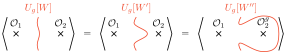
\includegraphics[width=\textwidth]{figures/tikz/Op_action.pdf}
\caption{The topological operator $U_g[W]$ is designed to be invariant under a continuous deformation and to implement the symmetry action.}
\label{fig-op-action}
\end{figure}

The construction is based on the concept of "cutting-and-gluing-with-twist".
Initially, we partition the spacetime $M$ into two subregions: $M_\stdim = M_L \cup_W M_R$ with a common boundary $W$ (refer to \ref{fig-cut-M}. We orient $W$ such that $\partial M_L = -\partial M_R = W$.).
We also divide the scalar field $\phi$ into two fields: $\phi_L(x)$ for $x \in M_L and \phi_R(x)$ for $x \in M_R$. Subsequently, we reconnect the two regions and their respective fields, with a twisted identification: 
\begin{equation}
\phi_L|_W = \phi_R^{g^{-1}}|_W.
\end{equation}

\begin{figure}[ht]
\centering
\includegraphics[width=.4\textwidth]{figures/tikz/ManifoldSplit.pdf}
\caption{The cutting and twisted gluing, implementing the topological operator $U_g[W]$.}
\label{fig-cut-M}
\end{figure}

In path-integral, this construction can be implemented as follows:

\begin{important}
{Symmetry Topological Operator for a Classical Symmetry}
\begin{equation}
\begin{multlined}
    \langle U_g[W] \cdots \rangle = \int \mathop{\mathcal{D}^{M_L}\phi_L} \mathop{\mathcal{D}^{M_R}\phi_R} \mathop{\mathcal{D}^W\lambda} \cdots\\ \times \exp\left(-S_L[\phi_L]-S_R[\phi_R] - G_W[\lambda,\phi_L,\phi_R,g]\right)
\end{multlined}
\label{eq-Ug-pathintegral}
\end{equation}
\end{important}

Here, $\mathcal{D}^{X}$ denotes the measure for the path-integral for a field defined on a submanifold $X$ of the spacetime $M$. The actions on the submanifold $M_{L,R}$ are written as $S_{L,R} = \int_{M_{L,R}}\mathcal{L}(\phi_{L,R})$, and "$\cdots$" denotes additional operator insertions. The "gluing" action $G_W$ on the submanifold $W$ is defined as
\begin{equation}
%\begin{multlined}
    G_W[\lambda,\phi_L,\phi_R,g] = - \imunit \int_W \lambda(\phi_L - \phi_R^{g^{-1}})\vol_W+\int_W s(\phi_R^{g^{-1}},g).
%\end{multlined}
\label{eq-gluing-action}
\end{equation}
The key point of the above expression is that integrating the Lagrange multiplier $\lambda$ results in the "delta functional":
\begin{equation}
    \int \mathop{\mathcal{D}^W\lambda} \exp\left(\imunit \int_W \lambda (\phi_L-\phi^{g^{-1}}_R)\vol_W\right)
     = \prod_{x\in W}\delta(\phi_L(x) - \phi_R^{g^{-1}}(x)),
\label{eq-delta-functional}
\end{equation}
which should implement \ref{fig-cut-M}.
Before studying the operator $U_g[W]$, we should first examine the \textit{trivial} case where the symmetry transformation $g$ is the identity map $g=\id$.
\begin{equation}
\langle \id[W] \cdots \rangle = \langle \cdots \rangle.
\label{eq-identity-wall}
\end{equation}
We refer to the codimension-1 operator $\id[W]$ with this property as the \textbf{identity wall}. It can also be termed as the \textbf{transparent wall} or similar.
Upon expanding \eqref{eq-identity-wall}, the following equation should be satisfied:
\begin{equation}
\begin{multlined}
    \int \mathop{\mathcal{D}^M\phi} \exp(-S) \cdots=
    \int \mathop{\mathcal{D}^{M_L}\phi_L} \mathop{\mathcal{D}^{M_R}\phi_R} \mathop{\mathcal{D}^W\lambda} \\ \times \exp\left(-S_L-S_R+\imunit \int_W \lambda(\phi_L - \phi_R)\vol_W\right)\cdots.\\ 
\end{multlined}
\label{eq-trivial-scalar}
\end{equation}

The key distinction between providing a field $\phi$ on $M$ and providing a pair of fields $(\phi_L,\phi_R)$ on $(M_L,M_R)$ is that the latter is not required to be continuous across $W$. On the right-hand side, continuity is enforced by integrating out $\lambda$ due to \eqref{eq-delta-functional}.


\begin{note}
{Continuity of Fields in "Exotic" QFTs and Subsystem Symmetry}
In this context, we assume that the path integral $\int\mathcal{D}^M\phi$ should be over the \emph{continuous} fields. This is because the standard kinetic term would diverge when the field $\phi$ becomes discontinuous, and thus such configuration does not contribute to the path-integral. 

However, this assumption does not hold for QFTs with higher-derivative kinetic terms. Examples of such exotic QFTs (without relativistic symmetry) include tensor gauge theories (refer to [@Pretko:2020cko;@Seiberg:2020bhn] for more details). An example of such kinetic term is $(\partial_t\phi)^2 + (\partial_x\partial_y \phi)^2$. In these theories, a field can be discontinuous, but some higher derivatives are constrained to scale appropriately with the ratio of the lattice size to the system size. In such scenarios, the construction of the trivial operator should differ.

These QFTs describe what is known as the \textbf{fracton} phases of matter, which do not have continuous rotational symmetry. Moreover, these models often possess \textbf{subsystem} symmetries, whose corresponding operator is not entirely topological. The existence of this new type of symmetry, absent in standard relativistic systems, is related to this subtlety regarding identity wall.
\end{note}

Let us study the equations of motion (EOMs) on the right-hand side of \eqref{eq-trivial-scalar}. The EOM with respect to $\lambda$ simply enforces $\phi_L(x) = \phi_R(x)$ for $x\in W$. On the other hand, the surface term of the Euler-Lagrange equation for $\phi_L$ and $\phi_R$ yields
\begin{equation}
    \left.\frac{\delta \mathcal{L}[\phi_L]}{\delta \mathop{d\phi_L}}\right|_W = \lambda \vol_W = \left. \frac{\delta \mathcal{L}[\phi_R]}{\delta \mathop{d \phi_R}}\right|_W.
\end{equation}
If $W$ is spacelike, or if we interpret the direction perpendicular to $W$ as the imaginary time in Euclidean signature, this condition ensures the continuity of the canonical momentum across $W$.

\begin{note}
{Locality}
\eqref{eq-trivial-scalar} encapsulates the \textbf{locality} of the path-integral. We can employ the same procedure to decompose the path-integral $\int \mathcal{D}^M{\phi}$ on $M$ into path-integrals on local patches, like $\int \prod_i\mathcal{D}^{V_i}\phi_i$ (accompanied by numerous Lagrange multipliers). Here, $\bigcup_i V_i =M$ and $V_i \cap V_j$ has codimension 1 in $M$ if not empty.

In the realm of topological quantum field theory (TQFT), a similar \textbf{cutting-and-gluing} axiom is utilized in the Atiyah-Segal formulation of topological quantum field theory. Later, Lurie's cobordism hypothesis \cite{Lurie} established the relationship between this axiom and locality.
\end{note}

%\begin{note}
%{A note on fermions}
%While this lecture does not cover fermions, it's worth noting how they would differ in this context.
%
%In scalar field theory, we enforce the continuity of the "position" variables (in the analytical-mechanical sense) $\phi$, and the continuity of the momentum variables follows from the equations of motion (EOM).
%
%However, in a chiral fermion theory, the kinetic term involves only one derivative, making it typically impossible to separate position and momentum variables while preserving Lorentz or global chiral symmetry.
%Consequently, the "cutting" process would seemingly violate invariance under Lorentz or another symmetry, which can be interpreted as a manifestation of the gravitational and global symmetry anomaly.
%A precise understanding of this perspective is beyond the scope of this lecture.
%\end{note}

\subsection{Topological-ness}
Let us show the topological-ness of $U_g$, i.e. the first equation in \ref{fig-op-action}, or
\begin{equation}
U_{g}[W_1]\id[W_2] = \id[W_1]U_{g}[W_2].
\label{eq-U-top}
\end{equation}
To show \eqref{eq-U-top}, we divide the spacetime into three parts: $M_L,M_M$ and $M_L$, where $W$ separates $M_L$ and $M_M$, while $W'$ separates $M_M$ and $M_R$.
The relevant part of path-integral regarding the left-hand side of \eqref{eq-U-top} reads
\begin{equation}
\int\mathcal{D}^{M_M}\phi_M\mathcal{D}^{W_1}\lambda_1\mathcal{D}^{W_2}\lambda_2 \, e^{-S_M[\phi_M]-G_{W_1}[\phi_L,\phi_M,g]-G_{W_2}[\phi_M,\phi_R,\id]}.
\end{equation}
Here $S_M = \int_{M_M}\mathcal{L}[\phi_M]$ and we omit the path-integral measures for $\phi_{L,R}$ and also the actions on $M_L$ and $M_R$ for the sake of readability.
By changing the variable by $\tilde{\phi}_M^{g} = \phi_M$, we get the expression
\begin{equation}
\int\mathcal{D}^{M_M}\tilde{\phi}_M^g\mathcal{D}^{W_1}\lambda_1\mathcal{D}^{W_2}\lambda_2 \, e^{-S_M[\tilde\phi_M^g]-G_{W_1}[\lambda_1,\phi_L,\phi_M,\id] - \int_{W_1} s(\tilde\phi_M,g) -G_{W_2}[\lambda_2,\tilde\phi_M^g,\phi_R,\id]}.
\end{equation}
As $M_M$ is open, the action $S_M[\tilde\phi_M^g]$ catches up the surface term:
\begin{equation}
S_M[\tilde\phi_M^g] = S_M[\tilde\phi_M] - \int_{W_1} s(\tilde{\phi}_M,g) + \int_{W_2} s(\tilde{\phi}_M,g).
\end{equation}
Using this equation combined with \eqref{eq-surface-term-inverse}, we get
\begin{equation}
\int\mathcal{D}^{M_M}\tilde{\phi}_M^g\mathcal{D}^{W_1}\lambda_1\mathcal{D}^{W_2}\lambda_2 \, e^{-S_M[\tilde\phi_M^g]-G_{W_1}[\lambda_1,\phi_L,\tilde\phi_M,\id] -G_{-W_2}[\lambda_2,\phi_R,\tilde\phi_M,g^{-1}]},
\end{equation}
where $-W_2$ is the orientation reversal of $W_2$.
Then we use the invariance of the path-integral measure of the scalar fields (up to the overall normalization):
\begin{equation}
\mathcal{D}^{M_M}\phi_M = \mathcal{D}^{M_M}\phi_M^g
\label{eq-measure-inv}
\end{equation}
to get
\begin{equation}
U_{g}[W_1]= U_{g^{-1}}[-W_2].
\end{equation}

Lastly, we need to show
\begin{equation}
U_{g^{-1}}[-W] = U_g[W].
\label{eq-Udual-inverse}
\end{equation}
To show this, we assume that there exists a transformation $\lambda^g$ of $\lambda$ that satisfies
\begin{equation}
\lambda(\phi_L-\phi_R) = \lambda^{g}(\phi_L^{g}-\phi_R^{g})
\end{equation}
and
\begin{equation}
\mathcal{D}^W\lambda^g = \mathcal{D}^W\lambda.
\end{equation}
For example, when the action is a $\U(1)$ rotation, $\lambda^g = g^{-1}\lambda$.
When the action is a shift of $\phi$, we can set $\lambda^g = \lambda$.
Under this assumption we get,
\begin{equation}
\begin{split}
U_{g^{-1}}[-W] &= \int\mathcal{D}^W \lambda \, e^{-G_{-W}[\lambda^{g^{-1}},\phi_R,\phi_L,g^{-1}]}\\
&= \int\mathcal{D}^W \lambda \, e^{\imunit\int_{-W}\lambda(\phi_R-\phi_L^{g})\vol_W - \int_{-W}s(\phi_L^{g},g^{-1})}\\
&= \int\mathcal{D}^W \lambda \, e^{\imunit\int_{W}\lambda^{g^{-1}}(\phi_L-\phi_R^{g^{-1}})\vol_W - \int_{W}s(\phi_L,g)}\\
&= \int\mathcal{D}^W \lambda^{g^{-1}} \, e^{-G_W[\lambda^{g^{-1}},\phi_L,\phi_R,g]}\\
&= U_g[W].
\end{split}
\end{equation}

We note that we can also get the following equation in the same way as above:
\begin{equation}
\langle \mathcal{O}_1 \mathcal{O}_2 \cdots \rangle = \langle U_g[W_0] \mathcal{O}_1 \mathcal{O}_2 \cdots \rangle,
\label{eq-bubble}
\end{equation}
when $W_0$ encloses a compact region of $M$ and contains no operator.

\subsection{}

\subsubsection*{Citation test}
\cite{Barkeshli:2014cna}
\subsection*{Acknowledgments}

\bibliographystyle{JHEP}
\bibliography{references}

\end{document}
